%%%%%%%%%%%%%%%%%%%%%%% file template.tex %%%%%%%%%%%%%%%%%%%%%%%%%
%
% This is a general template file for the LaTeX package SVJour3
% for Springer journals.          Springer Heidelberg 2010/09/16
%
% Copy it to a new file with a new name and use it as the basis
% for your article. Delete % signs as needed.
%
% This template includes a few options for different layouts and
% content for various journals. Please consult a previous issue of
% your journal as needed.
%
%%%%%%%%%%%%%%%%%%%%%%%%%%%%%%%%%%%%%%%%%%%%%%%%%%%%%%%%%%%%%%%%%%%
%
% First comes an example EPS file -- just ignore it and
% proceed on the \documentclass line
% your LaTeX will extract the file if required
\begin{filecontents*}{example.eps}
%!PS-Adobe-3.0 EPSF-3.0
%%BoundingBox: 19 19 221 221
%%CreationDate: Mon Sep 29 1997
%%Creator: programmed by hand (JK)
%%EndComments
gsave
newpath
  20 20 moveto
  20 220 lineto
  220 220 lineto
  220 20 lineto
closepath
2 setlinewidth
gsave
  .4 setgray fill
grestore
stroke
grestore
\end{filecontents*}
%
\RequirePackage{fix-cm}
%
%\documentclass{svjour3}                     % onecolumn (standard format)
%\documentclass[smallcondensed]{svjour3}     % onecolumn (ditto)
\documentclass[twocolumn]{svjour3}       % onecolumn (second format)
%\documentclass[twocolumn]{svjour3}          % twocolumn
%
\smartqed  % flush right qed marks, e.g. at end of proof
%

\usepackage{booktabs}
\usepackage{amsmath}
\usepackage[utf8]{inputenc} 
\usepackage{graphicx}
\usepackage{listings}
\usepackage{color}
\definecolor{dkgreen}{rgb}{0,0.6,0}
\definecolor{gray}{rgb}{0.5,0.5,0.5}
\definecolor{mauve}{rgb}{0.58,0,0.82}
\lstset{frame=tb,
  language=c,
  aboveskip=3mm,
  belowskip=3mm,
  showstringspaces=false,
  columns=flexible,
  basicstyle={\small\ttfamily},
  numbers=none,
  numberstyle=\tiny\color{gray},
  keywordstyle=\color{black},
  commentstyle=\color{dkgreen},
  stringstyle=\color{mauve},
  breaklines=true,
  breakatwhitespace=true,
  tabsize=3
}
\DeclareGraphicsExtensions{.pdf,.png,.jpg}
%
% \usepackage{mathptmx}      % use Times fonts if available on your TeX system
%
% insert here the call for the packages your document requires
%\usepackage{latexsym}
% etc.
%
% please place your own definitions here and don't use \def but
% \newcommand{}{}
%
% Insert the name of "your journal" with
% \journalname{myjournal}
%

\begin{document}
\title{Applying Multi-Core Model Checking to Hardware-Software Partitioning in Embedded Systems}
\author{Alessandro Trindade\and Hussama Ismail\and Renato Degelo\and Edilson Galv\~ao\and Lucas Cordeiro}
\institute{Electronic and Information Research Center\\Federal University of Amazonas, Brazil}
\maketitle

\begin{abstract}
We present an alternative approach to solve the hardware (HW) and software (SW) partitioning problem, which uses Bounded Model Checking (BMC) based on Satisfiability Modulo Theories (SMT) in conjunction with a multi-core support using Open MultiProcessing. The multi-core SMT-based BMC approach allows initializing many verification instances based on processors cores numbers available to the model checker. Each instance checks for a different optimum value until the optimization problem is satisfied. The goal is to show that multi-core model-checking techniques can be effective, in particular cases, to find the optimal solution of the HW-SW partitioning problem using an SMT-based BMC approach. We compare the experimental results of our proposed approach with Integer Linear Programming and the Genetic Algorithm.
\keywords{hardware-software co-design \and hardware-software partitioning\and optimization\and model checking\and multi-core\and OpenMP }
\end{abstract}

\section{Introduction}
Nowadays, with the strong development of embedded systems, the design phase plays an important role. At early stages, the design is split into separated flows: hardware and software. Consequently, the partitioning decision process, which deals with the decisions upon which parts of the application have to be designed in hardware (HW) and which in software (SW), must be supported by any well-structured methodology. If not, this leads to a number of issues (design flow interruptions, redesigns, and undesired iterations) which affects the overall development process, the quality and the lifecycle of the final system. Starting at the 1990s, intensive research was performed, and several approaches proposed, as shown in [1] and [2].

In any HW and SW design of complex systems, more time is spent on verification than on construction [3]. Formal methods based on model checking offer great potential to obtain a more effective and faster verification in the design process. Programs may be viewed as mathematical objects with behavior that is, in principle, well determined. This makes it possible to specify programs using mathematical logic, which constitutes the intended (correct) behavior. Then, one can try to give a formal proof or otherwise establish that the program meets its specification [4]. Research in formal methods has led to the development of very promising verification techniques, which facilitate the early detection of errors. Model-based verification techniques use models that describe the possible system behavior in a mathematically precise and unambiguous manner. The system models are accompanied by algorithms that systematically explore all the states of the system model.

In [5] and [6] was shown that it is possible to use Bounded Model Checking (BMC) based on Satisfiability Modulo Theories (SMT) to perform HW-SW partitioning in embedded systems. The present work extends those studies since there is a substantial improvement in terms of the genetic algorithm and the SMT-based verification method, which has been extended with a multi-core architecture. Multi-core processors have been used in all segments of industry to implement high-performance computing [7]. In particular, hardware platforms, together with multi-processing platforms, have allowed verification algorithms to distribute tasks executions across multiple processors, which generate an increase in performance if compared to single-core solution. However, most verification algorithms still disregard the limitations of the CMOS technology, which limits the increase of the chip’s frequency after it reaches 4 GHz.

Here, we exploit the availability of multi-core processors. In particular, a multi-core SMT-based BMC method is applied to the HW-SW partitioning and then is compared to the results with classical integer linear programming (ILP) and genetic algorithm (GA) using a multi-core tool as well. To the best of our knowledge, this is the first work to use a multi-core SMT-based verification to solve a HW-SW partitioning problem in embedded systems. We implement our ideas with the Efficient SMT-based Bounded Model Checker (ESBMC) tool [14]. As its main contribution, this paper shows that it is possible to take advantage of an SMT-based BMC tool in a multi-core architecture to solve optimization problems.

This paper is organized as follows: Section II gives a background on optimization, model checking, and multi-core support with Open MultiProcessing. Section III describes informal and formal mathematical modeling. Section IV describes briefly the binary integer programming and GA algorithms. The SMT-based BMC method is presented in Section V. Section VI presents the experimental evaluation. Section VII discusses related work. Section VIII presents the conclusion and future work.


\section{BACKGROUND}
\subsection{Optimization}
Optimization is the act of obtaining the best result (i.e., the optimal solution) under given circumstances [9]. In the design, construction, and maintenance of any engineering system, engineers have to make many technological and managerial decisions at several stages. The ultimate goal of all such decisions is either to minimize the effort required or to maximize the desired benefit. Because the effort required or the benefit desired in any practical situation can be expressed as a function of certain decision variables, optimization can be defined as the process of finding the conditions that give the maximum or minimum value of a function [9].

There is no single method available for solving all optimization problems efficiently [9]. The most known technique is linear programming, which is an method applicable for the solution of problems in which the objective function and the constraints appear as linear functions of the decision variables. A particular case of linear programming is ILP, in which the variables can assume just integer values. Eq. (1) shows a typical linear programming problem, where  and  are vectors or matrixes that describe the constraints
\begin{equation}
  minf^t x \: such that  = 
  \begin{cases}
    A.x \leq b, \\ 
    Aeq.x = beq, \\ 
    x \geq 0.
  \end{cases}
\end{equation}

In some cases, the time to find a solution using ILP is impractical. Even with the use of powerful computers, a problem can take hours running before an optimal solution is reached. If the optimization problem is complex, some heuristics can be used to solve the same problem faster, e.g., those used in the GA [9]. The only drawback is that the found solution may not be the global minimum or maximum.

\subsection{Optimization with Vz}
Um solucionador SMT e uma ferramenta com finalidade de verificar a satisfabilidade de formulas baseada em um conjunto de regras SMT. Z3 e um solucionador SMT da Microsoft Research, disponibilizado livremente para a comunidade que integra suporte para uma variedade de teorias. Z3 tras consigo um solucionador DPLL juntamente de uma máquina de correspondencia para quantificadores. Z3 e implementado em C++.

vZ e uma das ferramentas implementadas no solucionador Z3, a funcao base desta ferramenta e otimizar objetivos dentro do contexto logico das restricoes, este se destaca pelas funcoes que dao a possibilidade de formular criterios de otimizacao. 
vZ inclui uma versao incremental de MaxRes para MaxSAT e um Simplex para solucionar numeros sem padrao definido, em seu nucleo MaxSat e responsavel pelas restricoes enquanto OptSMT tem como funcao otimizar objetivos de aritmetica linear.
Dentre todos os avancos do Z3 usando vZ destaca-se as funcoes: maximize, minimize and assert-soft.
\begin{itemize}
\item{\textbf{maximize(T)}
esta instrucao diz ao solucionador que a variavel T devera ser maximizada, e possível maximizar valores reais, inteiros e vetores de bit.}
\item{\textbf{minimize(T)}
esta instrucao diz ao solucionador que a variavel T devera ser minimizada, os tipos aceitos pelo minimize e similar ao maximize.}
\item{\textbf{Assert-Soft F :weight n}
a instrucao Assert-soft e uma restricao sobre F, e possível adicionar um peso n, o padrão e 1.} 
\end{itemize}

Vamos otimizar (K+W), com restrições em (K \textless 2) e (W-K \textless 1), o resultado da otimização descrita no código abaixo é 2, o modelo gerado pelo vZ mostra que K = 1 e W =1.

\begin{lstlisting}
1. (declare-const K Int) 
2. (declare-const W Int)
3. (assert (< K 2)) 
4. (assert (< (- W K) 1))
5. (maximize (+ K W)) 
6. (check-sat)
\end{lstlisting}


De acordo com [34] a arquitetura do vZ pode ser descrita na imagem XXX, inicialmente as formulas e os objetivos SMT sao reescritos para variaveis do tipo 0-1, posteriormente os objetivos sao convertidos para problemas MaxSAT, se houver muitos objetivos vZ invoca MaxSAT ou OptSMT. Para restricoes sob valores reais usando “Box”, vZ combina todas a aritmetica linear e faz chamada para OptSMT. Quando usamos “soft constrains” no modo “lexicographic” vZ invoca MaxSAT.

\begin{figure}[ht]
	\centering
  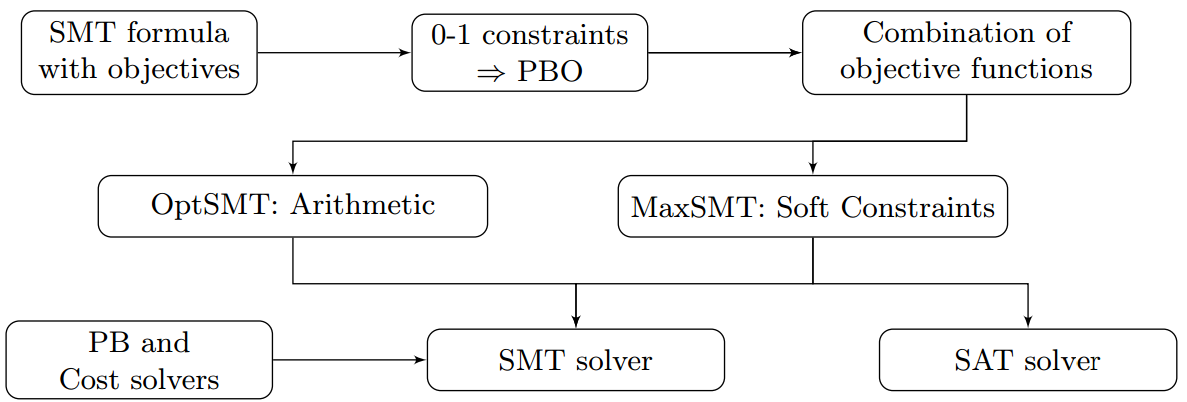
\includegraphics[width=0.49\textwidth, height=95px]{Image/vzArch.png} 
	\caption{vZ Architecture}
	\label{fig2}
\end{figure}


Z3 is available for platforms like C, C ++, Java, .NET and Python, it is possible to download the Z3 with vZ in http://z3.codeplex.com. API in python was used to formulate the optimization problem on the vZ tool. The pseudo code below describes the steps to achieve desired results.

\subsection{Bounded Model Checking with ESBMC}

Model checking refers to algorithms for exploring the state space of a transition system to determine if it obeys a specification of its intended behavior [3],[4]. These algorithms can perform exhaustive exploration in a highly automatic way and, thus, have attracted much interest in industry. However, model-checking has been held back by the state explosion problem, in which the number of states in a system grows exponentially in the number of system components [10]. Much research has been devoted to mitigate this problem.

Among the recent techniques, there is one that combines model checking with satisfiability solving. This technique, known as bounded model checking (BMC), does a very fast exploration of the state space, and for some types of problems, it offers large performance improvements over previous approaches, as shown in [10]. In particular, BMC based on Boolean Satisfiability (SAT) has been introduced as a complementary technique to binary decision diagrams for alleviating the state explosion problem. 

The basic idea of BMC is to check the negation of a given property at a given depth: given a transition system $ M $, a property $ \phi $, and a bound $ K $, BMC unrolls the system  times and translates it into a verification condition (VC) $ \varphi $  such that $ \varphi $   is satisfiable if and only if $ \phi $ has a counterexample of depth $ K $ or less [10]. To cope with increasing software complexity, SMT solvers can be used as back-ends for solving the generated VCs, as shown in [11], [12], and [13]. 

According to [14] and [15], SMT-based model checking can be used to verify the single- and multi-threaded software. In [16], ESBMC can also be used to model check C++ software based on SMT solvers. In [5] and [6] it was shown that it is possible to use ESBMC, as an optimization tool.
There are two directives in C/C++ that can be used to guide a model checker to solve an optimization problem: ASSUME and ASSERT. The directive ASSUME is responsible for ensuring the compliance of constraints (software costs), and the directive ASSERT controls the halt condition or code violation (minimum hardware cost). Then, with some C/C++ code, it is possible to guide ESBMC to solve optimization problems.

\subsection{Multi-core ESBMC with OpenMP}
\subsection{Multi-core ESBMC with OpenMP using Binary Search}
The original parallelization was made by continuously forking the instances of the ESBMC until the first violation is find. 

Since OpenMP only returns from a parallelized loop when every forked thread finishes, some processor could remain idle for some time.
\begin{figure}[ht]
	\centering
  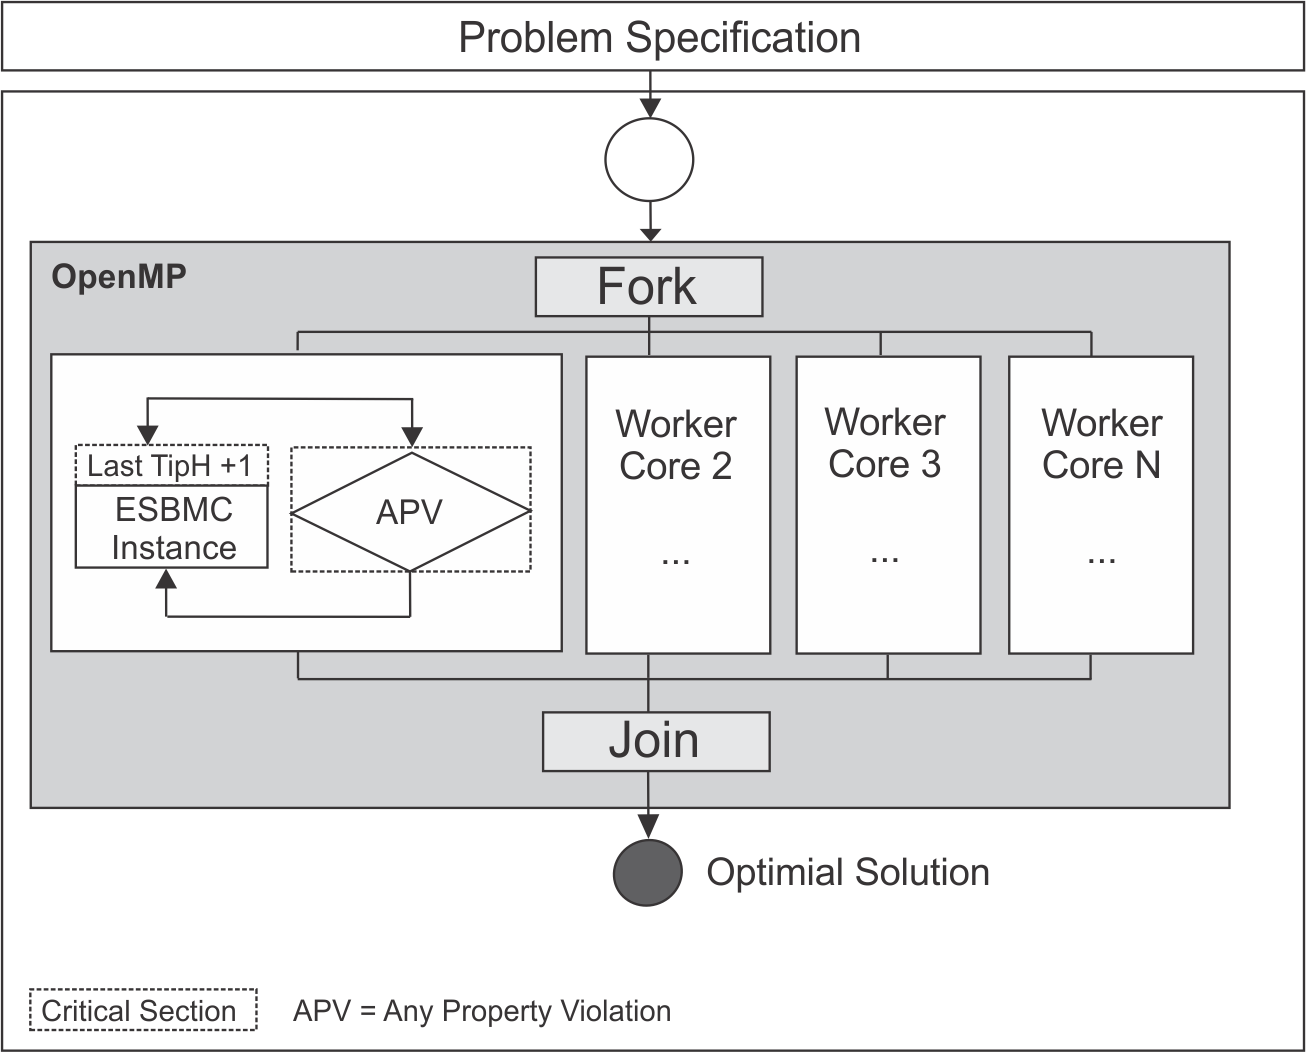
\includegraphics[scale=0.75]{Image/esbmc-parallel.png} 
	\caption{gestaucht}
	\label{fig2}
\end{figure}
So the first approach was to remove the Idle time from the parallel loops by creating workers inside the threads to always execute the next step until a violation is find. At first though it seemed to be a great improvement but as ESBMC executes almost the same time the steps, there was almost no optimization. 

The most optimized approach used was to use a parallelized binary search to reduce the complexity of the tasks. So was made a controller to return the best step to execute in order to reduce the domain as maximum as possible. This is done by dividing the domain in chunks and than returning the middle of the biggest chunk existent, and creating two new chunks.
\begin{figure}[ht]
	\centering
  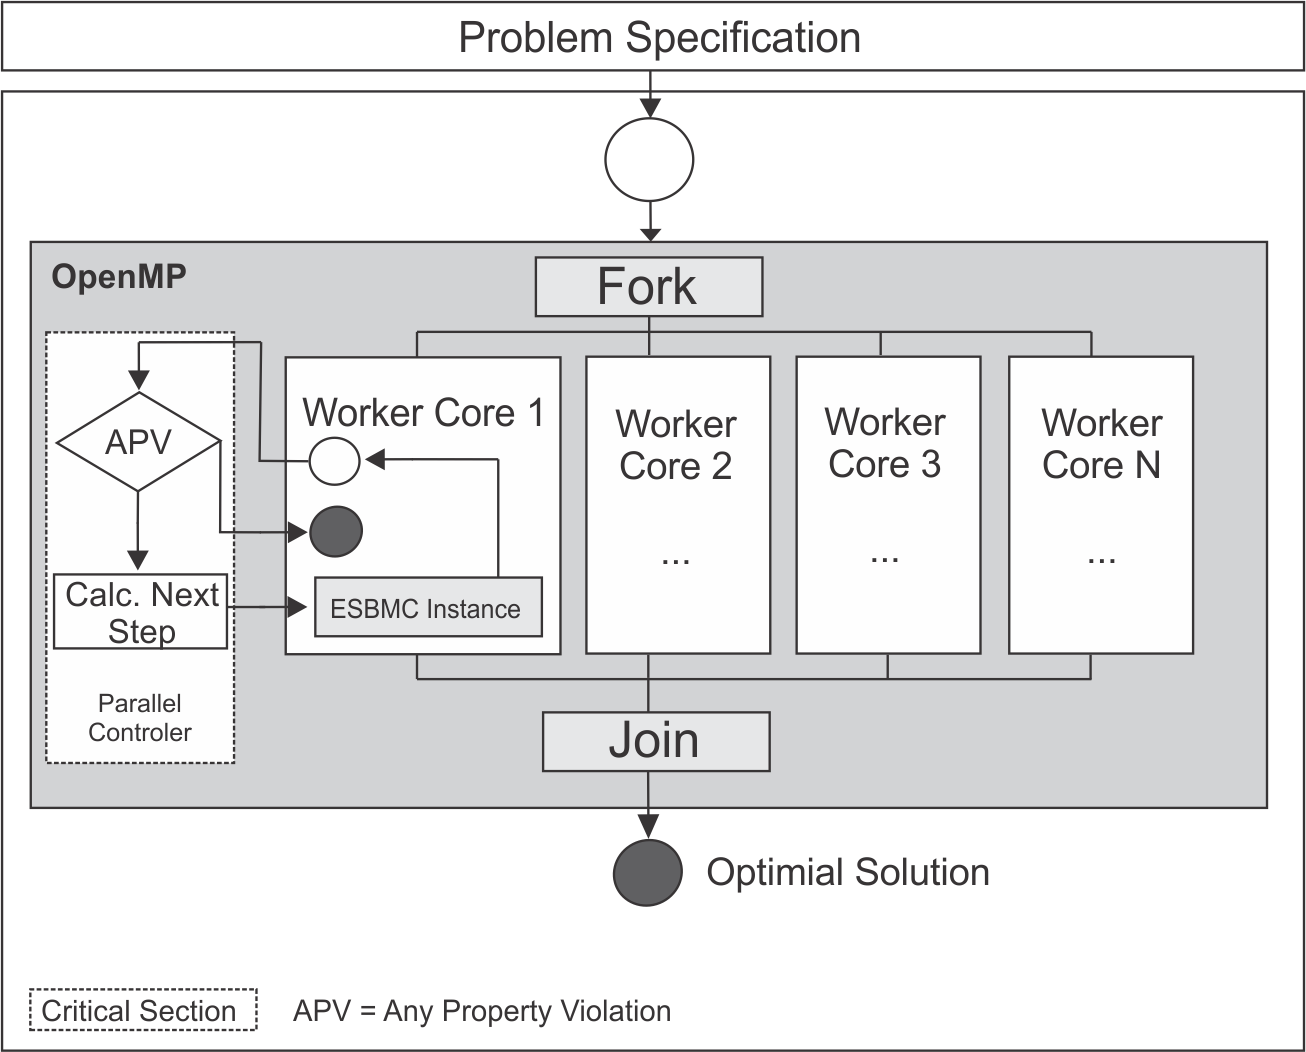
\includegraphics[scale=0.75]{Image/esbmc-parallel-Controler.png} 
	\caption{gestaucht}
	\label{fig2}
\end{figure}

To exemplify, given a problem of domain 1 to 20, first we create an initial chunk  1 – 20. When the next available core asks for a step to execute, the controller gets the biggest chunk which in this case is 1 – 20, divide it by 2, creates two new chunks and return the middle of the original chunk. So it would be 2 new chunks 1 – 9 and 11 – 20, and the returned step will be 10. Additional checks are needed to avoid the creation of empty or invalid chunks.
\begin{figure}[ht]
	\centering
  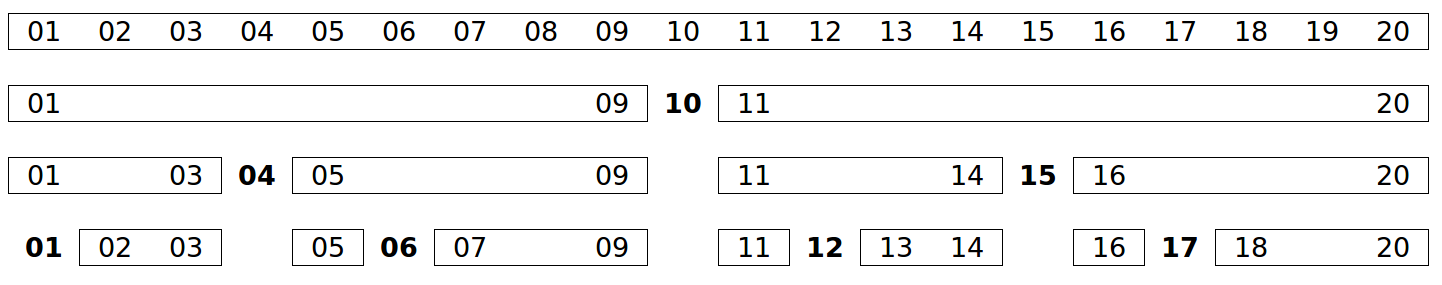
\includegraphics[width=0.49\textwidth, height=75px]{Image/Fig4.png}
	\caption{gestaucht}
	\label{fig2}
\end{figure}

Additionally, since there will be a gap between the steps, produced by the customized binary search algorithm, it is possible that a lot of steps will not be needed to execute. For instance, on the example above, if a step 10 return false, it is obvious that every step after 10 will also be a violation. On the other hand, if the same step was successful, we can assume that every step before 10 will also be a valid. 

That said, was implemented in the controller a method to discard unnecessary steps by removing or shrinking existing chunks. It made a very big impact in the calculation time. However a step can be running and not be needed anymore, in this case the binary algorithm kills the forked  process and starts a new one.
\begin{lstlisting}
01. GetNextStep(){
02.  int largestChunk = -1;
03.  chunk largest;
04.  for each(chunk in chunks){
05.     if(chunk.right - chunk.left > largestChunk){
06.           largestChunk = chunk.right - chunk.left;
07.           largest = chunk;
08.     }
09.   }	
10.   chunks.remove(largest);	
11.   int median = largest.left + floor((largest.right - largest.left) / 2)
12.   if(median > 0){
13.      if(largest.right - largest.left > 1)
14.         chunks.add(new chunk(largest.left, median - 1));	
15.      if(largest.right != largest.left)
16.         chunks.add(new chunk(median + 1, largest.right);
17.    }
18.   return median;
19. }
\end{lstlisting}
 The execution is made by executing the procedure described pseudocode before and then starting the process of the ESBMC to execute the returned step.
While the step is being executed the algorithm query the controller to check if this step is still needed. If not, the ESBMC instance is killed and the worker is free to start another step.

\begin{lstlisting}
01. step = controller.GetNextStep();
02. int pid = ExecuteStep(step);
03. while(isRunning(pid)){
04.   if(!controller.isNeeded(step))
05.    kill(pid);
06. }     
\end{lstlisting}

\section{Mathematical modeling}
The mathematical modeling was taken from [1], [2].
\subsection{Informal Model (or Assumptions)}
The informal model can be described by five characteristics. First, there is only one software context, i.e., there is just one general-purpose processor, and there is only one hardware context. The components of the system must be mapped to either one of these two contexts. Second, the software implementation of a component is associated with a software cost, which is the running time of the component. Third, the hardware implementation of a component has a hardware cost, which can be area, heat dissipation, and energy consumption. Fourth, based on the premise that hardware is significantly faster than software, the running time of the components in hardware is considered as zero. Finally, if two components are mapped to the same context, then there is no overhead of communication between them; otherwise, there is an overhead. The consequence of these assumptions is that scheduling does not need to be addressed in this work. Hardware components do not need scheduling, because the running time is assumed to be zero. Because there is only one processor, software components do not need to be scheduled as well. Therefore, the focus is only on the partitioning problem. That configuration describes a first-generation co-design, where the focus is on bipartitioning [17].

\subsection{Formal Model}
...

\section{Partitioning problem using ILP-based,Genetic Algorithms}
\label{ILPGA}
The ILP and GA were taken from [5] and [6]. Both use slack variables in order to be possible to represent the constraints and to use commercial tools. However, GA had improvements from the parameters of related studies in order to increase the solution accuracy without producing timeout. The tuning was performed by empirical tests and resulted in changing of three parameters, which are passed to function ga of MATLAB [18]: the population size was set from 300 to 500, the Elite count changed from 2 (default value) to 50, and the number of Generations changed from 100* NumberOfVariables (default) to 75.

\section{Analysis of the partitioning problem using ESBMC}
\section{Analysis of the partitioning problem using vZ}
O pseudocódigo abaixo mostra as condições aplicadas em ILP, GA e ESBMC convertida para a ferramenta vZ descrita em [34] e [35]. 

Um contexto do vZ é criado, este recebe as restrições e devolve um modelo caso exista uma solução para o conjunto de restrições.  Posteriormente são declarados a quantidade de nós, quantidade de arestas, o valor de , o custo de hardware, custo de software, custo de comunicação, e a matriz de incidência E.   

As declarações aritméticas descritas nas linhas 10, 11,12 e 13 do pseudocódigo é uma transcrição da formula $ S(1-x) + C|Ex| \leq S{0} $ descrita na seção III.B, é referente ao custo de software (SF). Observe que na linha 11 uma variável temporária chamada TMP é criada para representar $C|Ex|$  , é aplicado então um produto entre o valor absoluto de TMP com o valor do vetor C declarado na linha 07, logo, gera-se o resultado para o custo de comunicação (CMC). 
Na linha 13, a declaração Fobj (Função objetivo) é um produto entre o custo de hardware com um vector que contém valores 0 ou 1. Fobj deve ser minimizado para alcançarmos a melhor solução para o hardware.

Duas restrições são impostas, a primeira refere-se à soma entre custo de software com o custo de comunicação, a resultante da soma deve ser menor do que , a segunda restrição diz ao vZ que ele deverá minimizar Fobj. O modelo então é checado, uma vez que há uma solução que obedeça às restrições, o valor da função objetiva é impressa. 

\begin{lstlisting}
01.#Init Values
02.  Create vZ context 
03.  Create binary vector (x)
04.  Declare number of nodes, edges and S0
05.  Declare hardware cost of each node as array (h) 
06.  Declare software cost of each node as array (s)
07.  Declare communication cost of each edge (c)
08.  Declare transposed incidence matrix graph G (E)
09.#Arithmetic
10.  SF receive s(1-x)
11.  TMP vector receive E|x| 
12.  CMC receive c*|EX|
13.  Fobj receive  x[i] * h[i]
14.#Asserts
15.  Add restrictions (SF + CMC <= S0)
16.  Add restrictions to minimize Fobj
17.  Check Model
18.  Print Result
\end{lstlisting}

\section{Experimental Evaluation}


\section{Related Work}
Since the second half of the first decade of the 2000s, three main paths have been tracked to improve or to present alternative solutions to the optimization of HW-SW partitioning, i.e., to find the exact solution [2], to use heuristics to speed up performance time [1], and hybrid ones [22].

In the first group, the exact solution to the HW-SW partitioning problem is found. The use of SMT-based verification presented in this paper can be grouped into this category, because the exact solution is found with the given algorithm. The difference is based only in terms of the technique chosen to solve the problem.
Another path followed in past initiatives and which has had more studies is the creation of heuristics to speed up the running time of the solution. The difference between this kind of solutions and SMT-based verification is based on two facts: ESBMC is guaranteed to find the exact solution, but the heuristics are faster when the complexity is greater.

Finally, there are approaches that mixes heuristics with exact solution tools. The idea is to use a heuristic to speed up some phase of an exact solution tool. It worth mentioning that the final solution is not necessarily an optimal global solution. Only the SMT-based verification is guaranteed to find the exact solution, but hybrid algorithms are faster when complexity rises.

In terms of SMT-based verification, most work is restricted to present the model, its modification to programming languages (e.g., C/C++ and Java), and the application to multi-thread algorithms or to embedded systems to check for program correctness. In [16] it presents a bounded model checker for C++ programs, which is an evolution of dealing with C programs and [14] uses the ESBMC model checker for embedded ANSI-C software. In [5] and [6] it was proven that it is possible to use ESBMC to solve HW-SW partitioning, but in a single core way. There are related studies focused on decreasing the verification time of model checkers by applying Swarm Verification [29], and modifications of internal search engines to support parallelism [30], but there is still the need for initiatives related to parallel SMT solvers [31]. Recently, the SMT solver Z3 has been extended to pose and solve optimization problems modulo theories [32].
\section{Conclusions}
Concerning the comparative tests, with the four techniques presented in this paper to solve HW-SW partitioning, it was evident that none of them is indicated to partition problems with more than 400 nodes. The computing time to solve the optimization problem reached some hours of execution on a standard desktop computer. If we consider less than 400 nodes, then it is possible to use ILP as the best solution provider. If the problem to be solved has 150 nodes or less, then ESBMC represents a feasible alternative. GA had an intermediate result in terms of performance, but the error presented from exact solution made it not acceptable to that kind of application. This error may be reduced by changing some parameters.

If considering off-the-shelf tools, as MATLAB to ILP and GA, the coding is simpler. However, ESBMC has a BSD-style license and can be downloaded and used for free. Concerning the two versions of ESBMC, it is possible to conclude that Multi-core ESBMC had better performance results than pure ESBMC. Thus, considering that nowadays the processors have more and more cores, when modeling the problem, it is possible to consider multi-core ESBMC as an alternative to solve the partitioning problem. Future work can be done to decrease the processing time of ESBMC (solver included).

Finally, there is an issue about 150 nodes problem, since it seems to be the limit of ESBMC. It really depends on the modeling granularity of the problem. Some researchers propose fine-grained models, in which each instruction can be mapped to either HW or SW. This may lead to thousands of nodes or even more. Others defend coarse-grained models, where decisions are made for bigger components, thus even complex systems may consist of just some dozens of nodes to partition. In principle, a fine-grained approach may allow to obtain better partitions, but at the cost of an exponential increase of the size of the search space. In future work, we will exploit other search strategies in the multi-core ESBMC approach and address specifically more complex types of architectures in the HW-SW partitioning problem, including more than one CPU.
\section{References}


\end{document}


% end of file template.tex

